\documentclass[11pt, a4paper]{article}

\usepackage[margin=1in]{geometry} % Set margins.
\usepackage{enumitem} % Customize lists.
\usepackage{hyperref} % For hyperlinks.
\usepackage{titlesec} % Custom section titles.
\usepackage{graphicx} % Required for including images
\usepackage{float} % For precise placement of the figure
\usepackage{fontawesome} % For icons
\usepackage{adjustbox}
\usepackage{tikz}


% Set section title formatting
\titleformat{\section}
{\large\bfseries} % Format
{} % Label
{0em} % Sep
{} % Before-code
[\titlerule] % After-code

\pagestyle{empty} % No page numbers

\begin{document}
\noindent
\begin{minipage}{0.25\textwidth}
    \begin{tikzpicture}
        % Define variables
        \def\xCenter{-0.1} % X center of the circle
        \def\yCenter{0.65} % Y center of the circle
        \def\circleRadius{1.9} % Radius of the circle
        
        % Clipping for the image
        \clip (\xCenter,\yCenter) circle (\circleRadius cm);
        
        % Place the image
        \node at (0, 0) {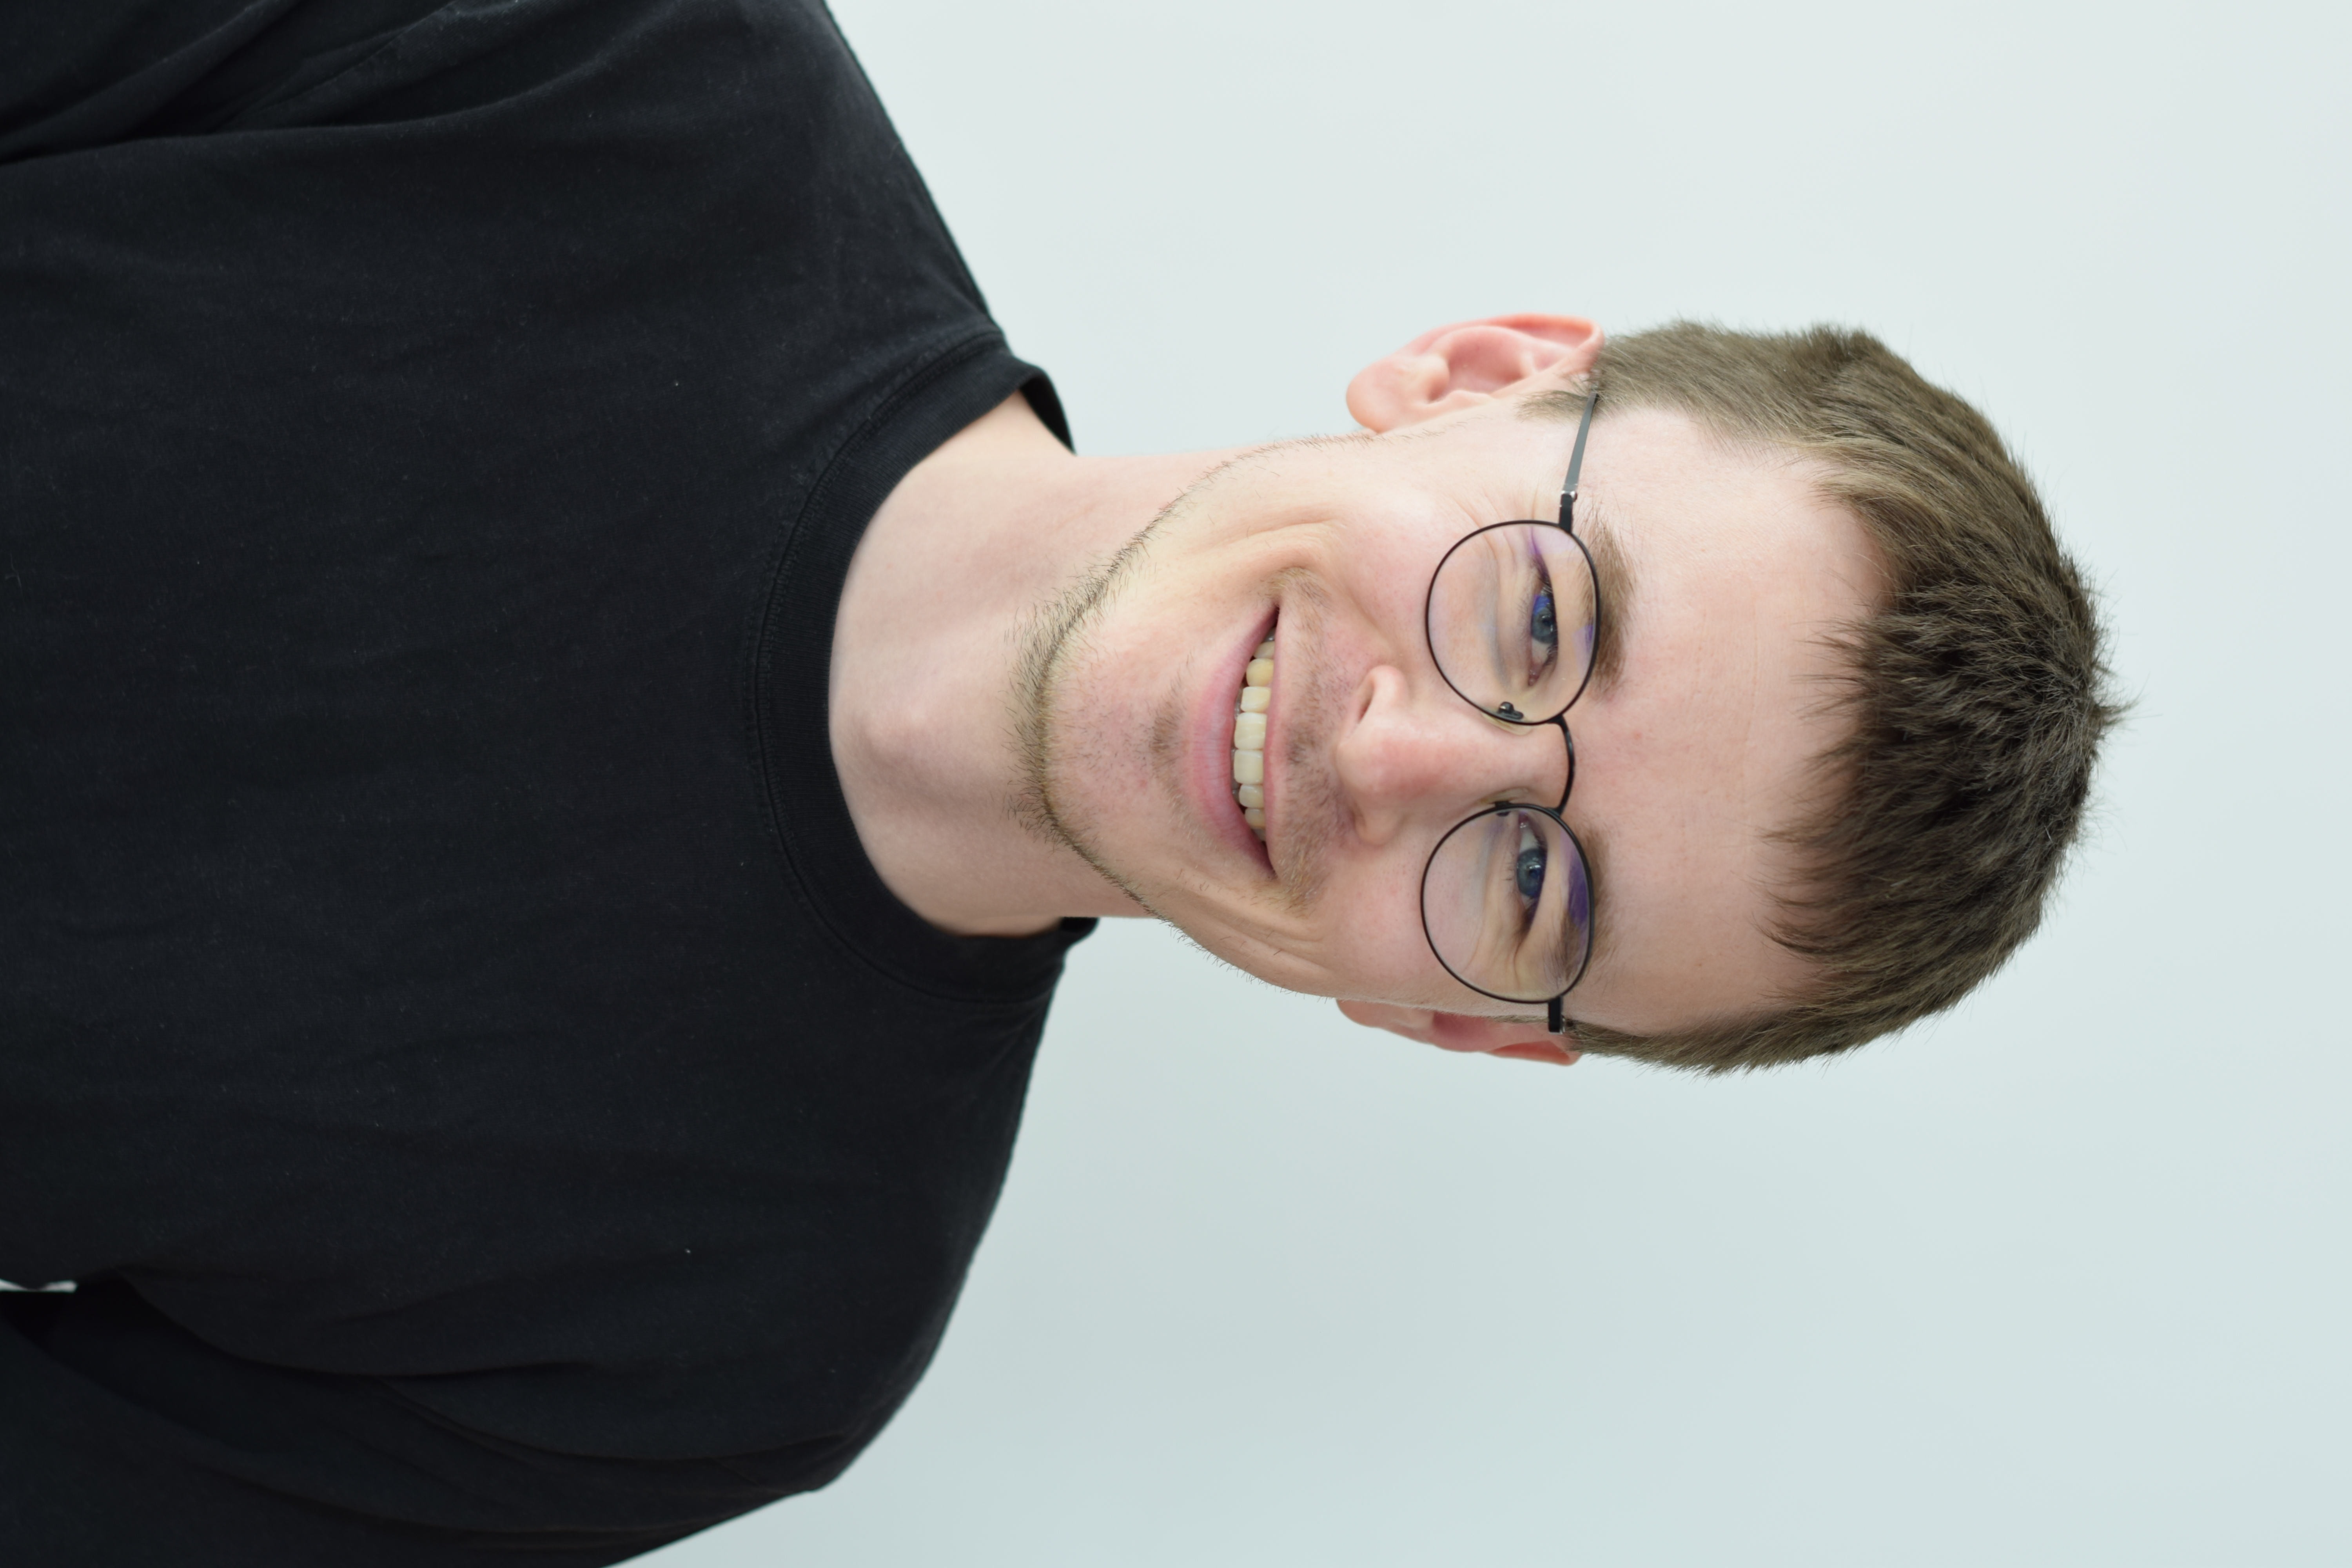
\includegraphics[height=4cm,angle=90]{./assets/profile_pic.jpg}};
        
        % Draw the circular border
        \draw[gray, thick] (\xCenter,\yCenter) circle (\circleRadius cm); % Adjust 'thick' as needed for border width
    \end{tikzpicture}

\end{minipage}%
\begin{minipage}{0.75\textwidth}
    \centerline{
        \Large\bfseries Frej Sundqvist
    }
    \vspace{0.2em}
    \centerline{
        \textit{Problem solver, Programmer, Engineer}
    }
    \centerline{
        From Sweden, living in Norway
    }
    \vspace{0.5em}
    \centerline{
        {\faEnvelopeO} \href{mailto:frejsundqvist@protonmail.com}{frejsundqvist@protonmail.com}
        |
        % target="_blank" to open in new tab
        {\faGithub} \href{https://github.com/MyosQ}{MyosQ}
    }
    \centerline{
        {\faLinkedin} \href{https://linkedin.com/in/frej-sundqvist-b8a49a14b}{frej-sundqvist-b8a49a14b}
        |
        {\faGlobe} \href{https://myosq.github.io/cv}{myosq.github.io/cv}    
    }
\end{minipage}

\vspace{1em}

\section*{Experience}
\textbf{Fullstack developer, Sysadmin, Tech lead, Project leader}, \textit{Capia AS}, Tromsø, Norway \hfill 2021 - Present
\begin{itemize}[noitemsep]
    \item Building applications from scratch to deployment.
    \item Leading teams of developers and interacting directly with customers.
    \item Fine-tuning Neural Networks for image segmentation and classification.
    \item System administering of servers and databases.
\end{itemize}

\section*{Education}
\textbf{Master's degree in Engineering Physics}
\begin{itemize}[noitemsep]
    \item Umeå university, Sweden \hfill 2015 - 2021
    \item Julius-Maximilians-Universität, Würzburg, Germany \hfill 2018 - 2019
\end{itemize}

\section*{Skills}
\begin{itemize}[noitemsep]
    \item Python, C, JavaScript, Rust, R, Matlab, PHP, 
    \item Pytorch, Pandas, Numpy,
    \item Django, React, Nodejs, 
    \item Git, Docker, Docker-compose, Kubernetes, Github/Bitbucket CI/CD,
    \item SQL, MariaDB, PostgreSQL, PostGis, Redis,
    \item Bash, Nginx,
    \item Google Cloud, Cloudflare, Backblaze,
    \item Apache Airflow, Kafka,
    \item HTML, CSS, LESS, 
    \item Linux System Administration, Network protocols,
\end{itemize}

% \section*{Projects}
% \textbf{Project Name}, \textit{Company Name}, Location \hfill Month Year – Month Year
% \begin{itemize}[noitemsep]
%     \item Description.
%     \item Another bullet point.
%     \item Another bullet point.
% \end{itemize}

\section*{Languages}
\begin{itemize}[noitemsep]
    \item Swedish: Native
    \item English: Fluent
    \item German: Fluent
    \item Norwegian: Fluent
\end{itemize}

\end{document}

\end{document}